%!TEX root = ../index.tex

Es dauerte einige Zeit, bis der Termin das Kick-Off Meeting gesetzt war. Dies lag unter anderem daran, dass zu Beginn dieser Arbeit gerade Semesterferien waren. Nachdem die Aufgabenstellung abgesegnet wurde, habe ich die Einzelnen Phasen des Projekts geschätzt und anhand dieser Schätzung einen Projektplan aufgestellt. Die Planungsphase fand vor dem Kick-Off Meeting statt. In dieser Phase wurde die Idee für diese Bachelorthesis ausgearbeitet, die Aufgabenstellung erfasst und eine Betreuungsperson gesucht. In der Einarbeitungsphase ging es vor allem darum, sich in vorhandene Literatur zum Thema einzulesen. Während der Katalogisierungsphase habe ich die häufigsten Fehlerszenarios katalogisiert in dem ich auch Entwickler von anderen Firmen befragt habe. Die Konzeptionierung Phase wurden die Fehlerszenarios Kategorisiert, die Anforderungen aufgenommen und Produkte evaluiert. Die folgende Proof of Concept Phase wurde genutzt um die Evaluierten Produkte in der allink einzuführen und die Eigenentwicklungen in Form eines Prototypen zu Programmieren. Die zwei letzten Phasen sind für die Fertigstellung der Dokumentation und für die Vorbereitungen für die Abschlusspräsentation vorgesehen.

\begin{table}[h]
  \centering
  \begin{tabular}{ll}
  \toprule
    Phase & Zeitschätzung\\
  \hline
    Planung & 40h\\
  \hline
    Einarbeitung & 40h\\
  \hline
    Katalogisierung & 70h\\
  \hline
    Konzeptionierung & 70h\\
  \hline
    Proof of Concept & 60h\\
  \hline
    Dokumentation & 60h\\
  \hline
    Präsentation & 20h\\
  \bottomrule
  \end{tabular}
  \caption{Zeitschätzung der einzelnen Phasen}
  \label{tab:zeitschätzung}
\end{table}


\begin{figure}[p]
\centering
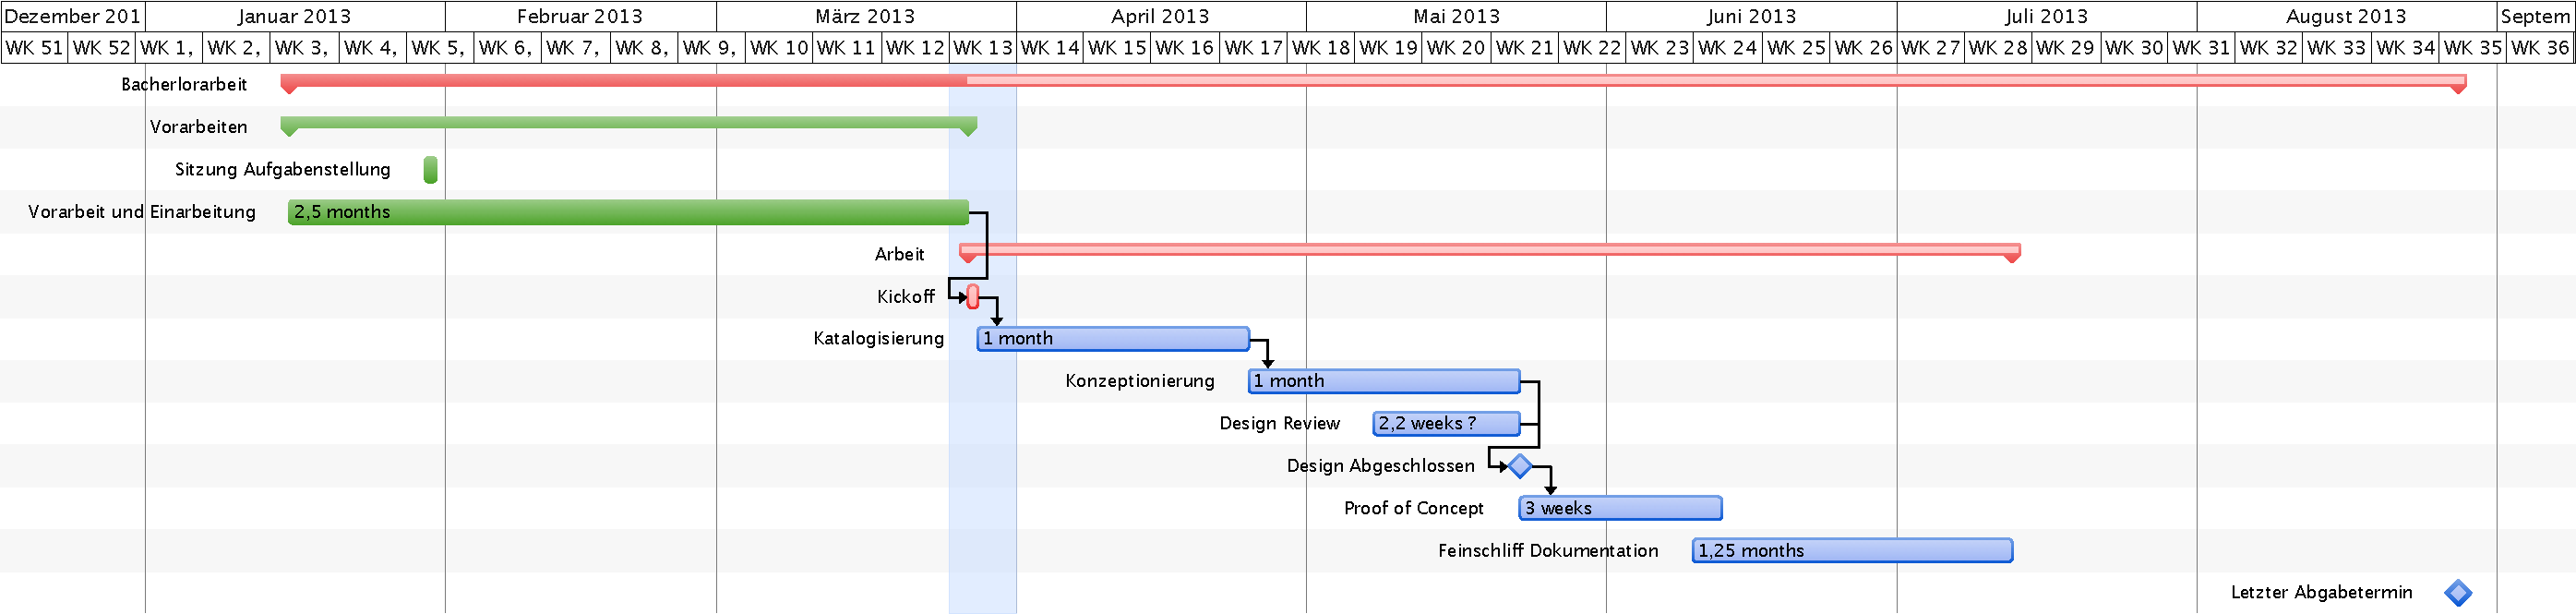
\includegraphics[width=1\textheight, angle=90]{images/projektplan.pdf}
\caption{Projektplan Stand Kick-Off}
\label{fig:projektplan}
\end{figure}

\section{Termine}
\label{sec:termine}
In der Tabelle~\ref{tab:sitzungen} werden alle Sitzungen aufgeführt welche im Rahmen dieser Arbeit gehalten wurden.

\begin{table}[h]
  \centering
  \begin{tabular}{lll p{7cm}}
  \toprule
    Datum & Ort & Thema & Anwesende Personen\\
  \hline
    31.1.2013 & ZHAW & Vorbesprechung Kick-Off & Beat Seeliger\\
  \hline
    27.3.2013 & ZHAW & Kick-Off & Dr. Reto Knaack, Beat Seeliger, Silvan Spross\\
  \hline
    17.4.2013 & Panter & Zwischenbesprechung & Beat Seeliger\\
  \hline
    22.5.2013 & ZHAW & Design-Review & Beat Seeliger, Silvan Spross\\
  \hline
    22.6.2013 & ZHAW & Zwischenbesprechung & Beat Seeliger\\
  \bottomrule
  \end{tabular}
  \caption{Sitzungen}
  \label{tab:sitzungen}
\end{table}

\section{Versionsverwaltung}
\label{sec:versionsverwaltung}
Um Änderungen am dieser Dokumentation zu verfolgen, habe ich seit Beginn dieser Arbeit diese mit der Versionsverwaltungssoftware Git\footnote{Frei verfügbar unter \url{http://git-scm.com/}} versioniert. Diese ganze Arbeit ist öffentlich unter nachfolgender \acrshort{url} erreichbar:

\url{https://github.com/frog32/bachelorarbeit}

Ebenfalls der Prototyp für den Statusmonitor wurde als Opensource Software entwickelt. Das zugehörige Git Repository ist ebenfalls öffentlich erreichbar:

\url{https://github.com/frog32/status-monitor}

